% Created by tikzDevice version 0.12 on 2020-02-07 10:56:33
% !TEX encoding = UTF-8 Unicode
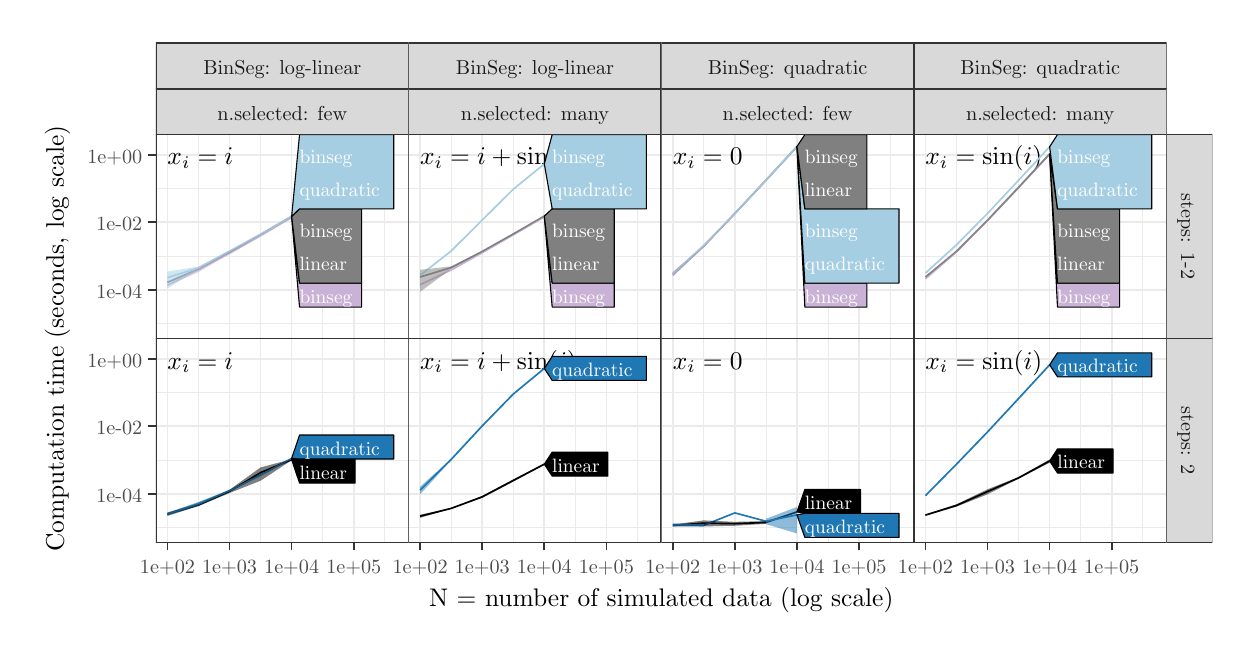
\begin{tikzpicture}[x=1pt,y=1pt]
\definecolor{fillColor}{RGB}{255,255,255}
\path[use as bounding box,fill=fillColor,fill opacity=0.00] (0,0) rectangle (433.62,216.81);
\begin{scope}
\path[clip] (  0.00,  0.00) rectangle (433.62,216.81);
\definecolor{drawColor}{RGB}{255,255,255}
\definecolor{fillColor}{RGB}{255,255,255}

\path[draw=drawColor,line width= 0.6pt,line join=round,line cap=round,fill=fillColor] (  0.00,  0.00) rectangle (433.62,216.81);
\end{scope}
\begin{scope}
\path[clip] ( 46.36,104.43) rectangle (137.66,178.17);
\definecolor{fillColor}{RGB}{255,255,255}

\path[fill=fillColor] ( 46.36,104.43) rectangle (137.66,178.17);
\definecolor{drawColor}{gray}{0.92}

\path[draw=drawColor,line width= 0.3pt,line join=round] ( 46.36,109.94) --
	(137.66,109.94);

\path[draw=drawColor,line width= 0.3pt,line join=round] ( 46.36,134.31) --
	(137.66,134.31);

\path[draw=drawColor,line width= 0.3pt,line join=round] ( 46.36,158.68) --
	(137.66,158.68);

\path[draw=drawColor,line width= 0.3pt,line join=round] ( 61.73,104.43) --
	( 61.73,178.17);

\path[draw=drawColor,line width= 0.3pt,line join=round] ( 84.17,104.43) --
	( 84.17,178.17);

\path[draw=drawColor,line width= 0.3pt,line join=round] (106.61,104.43) --
	(106.61,178.17);

\path[draw=drawColor,line width= 0.3pt,line join=round] (129.05,104.43) --
	(129.05,178.17);

\path[draw=drawColor,line width= 0.6pt,line join=round] ( 46.36,122.13) --
	(137.66,122.13);

\path[draw=drawColor,line width= 0.6pt,line join=round] ( 46.36,146.50) --
	(137.66,146.50);

\path[draw=drawColor,line width= 0.6pt,line join=round] ( 46.36,170.87) --
	(137.66,170.87);

\path[draw=drawColor,line width= 0.6pt,line join=round] ( 50.51,104.43) --
	( 50.51,178.17);

\path[draw=drawColor,line width= 0.6pt,line join=round] ( 72.95,104.43) --
	( 72.95,178.17);

\path[draw=drawColor,line width= 0.6pt,line join=round] ( 95.39,104.43) --
	( 95.39,178.17);

\path[draw=drawColor,line width= 0.6pt,line join=round] (117.83,104.43) --
	(117.83,178.17);
\definecolor{drawColor}{RGB}{0,0,0}

\node[text=drawColor,anchor=base west,inner sep=0pt, outer sep=0pt, scale=  0.92] at ( 50.51,167.21) {$x_i = i$};
\definecolor{drawColor}{RGB}{202,178,214}

\path[draw=drawColor,line width= 0.6pt,line join=round] ( 50.51,123.75) --
	( 61.73,129.32) --
	( 72.95,135.26) --
	( 84.17,141.64) --
	( 95.39,148.23);
\definecolor{drawColor}{gray}{0.50}

\path[draw=drawColor,line width= 0.6pt,line join=round] ( 50.51,124.78) --
	( 61.73,129.63) --
	( 72.95,135.78) --
	( 84.17,142.11) --
	( 95.39,148.60);
\definecolor{drawColor}{RGB}{166,206,227}

\path[draw=drawColor,line width= 0.6pt,line join=round] ( 50.51,126.47) --
	( 61.73,130.03) --
	( 72.95,136.04) --
	( 84.17,142.14) --
	( 95.39,148.64);
\definecolor{fillColor}{RGB}{202,178,214}

\path[fill=fillColor,fill opacity=0.50] ( 50.51,123.88) --
	( 61.73,130.10) --
	( 72.95,135.41) --
	( 84.17,141.68) --
	( 95.39,148.42) --
	( 95.39,148.04) --
	( 84.17,141.60) --
	( 72.95,135.10) --
	( 61.73,128.41) --
	( 50.51,123.62) --
	cycle;
\definecolor{fillColor}{RGB}{127,127,127}

\path[fill=fillColor,fill opacity=0.50] ( 50.51,124.93) --
	( 61.73,129.70) --
	( 72.95,136.00) --
	( 84.17,142.16) --
	( 95.39,148.62) --
	( 95.39,148.57) --
	( 84.17,142.06) --
	( 72.95,135.55) --
	( 61.73,129.55) --
	( 50.51,124.63) --
	cycle;
\definecolor{fillColor}{RGB}{166,206,227}

\path[fill=fillColor,fill opacity=0.50] ( 50.51,128.69) --
	( 61.73,130.47) --
	( 72.95,136.46) --
	( 84.17,142.17) --
	( 95.39,148.69) --
	( 95.39,148.58) --
	( 84.17,142.11) --
	( 72.95,135.58) --
	( 61.73,129.56) --
	( 50.51,122.59) --
	cycle;
\end{scope}
\begin{scope}
\path[clip] ( 46.36,104.43) rectangle (137.66,178.17);
\definecolor{drawColor}{RGB}{0,0,0}
\definecolor{fillColor}{RGB}{202,178,214}

\path[draw=drawColor,line width= 0.4pt,line join=round,line cap=round,fill=fillColor] ( 95.39,148.23) --
	( 98.24,124.52) --
	(120.67,124.52) --
	(120.67,115.85) --
	( 98.24,115.85) --
	cycle;
\definecolor{fillColor}{gray}{0.50}

\path[draw=drawColor,line width= 0.4pt,line join=round,line cap=round,fill=fillColor] ( 95.39,148.60) --
	( 98.24,151.35) --
	(120.67,151.35) --
	(120.67,124.52) --
	( 98.24,124.52) --
	cycle;
\definecolor{fillColor}{RGB}{166,206,227}

\path[draw=drawColor,line width= 0.4pt,line join=round,line cap=round,fill=fillColor] ( 95.39,148.64) --
	( 98.24,178.17) --
	(132.27,178.17) --
	(132.27,151.35) --
	( 98.24,151.35) --
	cycle;
\definecolor{drawColor}{RGB}{255,255,255}

\node[text=drawColor,anchor=base west,inner sep=0pt, outer sep=0pt, scale=  0.70] at ( 98.24,117.29) {binseg};

\node[text=drawColor,anchor=base west,inner sep=0pt, outer sep=0pt, scale=  0.70] at ( 98.24,141.09) {binseg};

\node[text=drawColor,anchor=base west,inner sep=0pt, outer sep=0pt, scale=  0.70] at ( 98.24,128.99) {linear};

\node[text=drawColor,anchor=base west,inner sep=0pt, outer sep=0pt, scale=  0.70] at ( 98.24,167.91) {binseg};

\node[text=drawColor,anchor=base west,inner sep=0pt, outer sep=0pt, scale=  0.70] at ( 98.24,155.82) {quadratic};
\definecolor{drawColor}{gray}{0.20}

\path[draw=drawColor,line width= 0.6pt,line join=round,line cap=round] ( 46.36,104.43) rectangle (137.66,178.17);
\end{scope}
\begin{scope}
\path[clip] ( 46.36, 30.69) rectangle (137.66,104.43);
\definecolor{fillColor}{RGB}{255,255,255}

\path[fill=fillColor] ( 46.36, 30.69) rectangle (137.66,104.43);
\definecolor{drawColor}{gray}{0.92}

\path[draw=drawColor,line width= 0.3pt,line join=round] ( 46.36, 36.20) --
	(137.66, 36.20);

\path[draw=drawColor,line width= 0.3pt,line join=round] ( 46.36, 60.57) --
	(137.66, 60.57);

\path[draw=drawColor,line width= 0.3pt,line join=round] ( 46.36, 84.94) --
	(137.66, 84.94);

\path[draw=drawColor,line width= 0.3pt,line join=round] ( 61.73, 30.69) --
	( 61.73,104.43);

\path[draw=drawColor,line width= 0.3pt,line join=round] ( 84.17, 30.69) --
	( 84.17,104.43);

\path[draw=drawColor,line width= 0.3pt,line join=round] (106.61, 30.69) --
	(106.61,104.43);

\path[draw=drawColor,line width= 0.3pt,line join=round] (129.05, 30.69) --
	(129.05,104.43);

\path[draw=drawColor,line width= 0.6pt,line join=round] ( 46.36, 48.39) --
	(137.66, 48.39);

\path[draw=drawColor,line width= 0.6pt,line join=round] ( 46.36, 72.76) --
	(137.66, 72.76);

\path[draw=drawColor,line width= 0.6pt,line join=round] ( 46.36, 97.13) --
	(137.66, 97.13);

\path[draw=drawColor,line width= 0.6pt,line join=round] ( 50.51, 30.69) --
	( 50.51,104.43);

\path[draw=drawColor,line width= 0.6pt,line join=round] ( 72.95, 30.69) --
	( 72.95,104.43);

\path[draw=drawColor,line width= 0.6pt,line join=round] ( 95.39, 30.69) --
	( 95.39,104.43);

\path[draw=drawColor,line width= 0.6pt,line join=round] (117.83, 30.69) --
	(117.83,104.43);
\definecolor{drawColor}{RGB}{0,0,0}

\node[text=drawColor,anchor=base west,inner sep=0pt, outer sep=0pt, scale=  0.92] at ( 50.51, 93.47) {$x_i = i$};

\path[draw=drawColor,line width= 0.6pt,line join=round] ( 50.51, 41.05) --
	( 61.73, 44.34) --
	( 72.95, 49.28) --
	( 84.17, 56.04) --
	( 95.39, 60.70);
\definecolor{drawColor}{RGB}{31,120,180}

\path[draw=drawColor,line width= 0.6pt,line join=round] ( 50.51, 41.11) --
	( 61.73, 44.85) --
	( 72.95, 49.50) --
	( 84.17, 55.14) --
	( 95.39, 61.16);
\definecolor{fillColor}{RGB}{0,0,0}

\path[fill=fillColor,fill opacity=0.50] ( 50.51, 41.64) --
	( 61.73, 44.70) --
	( 72.95, 49.84) --
	( 84.17, 57.91) --
	( 95.39, 60.87) --
	( 95.39, 60.52) --
	( 84.17, 53.11) --
	( 72.95, 48.66) --
	( 61.73, 43.96) --
	( 50.51, 40.37) --
	cycle;
\definecolor{fillColor}{RGB}{31,120,180}

\path[fill=fillColor,fill opacity=0.50] ( 50.51, 41.52) --
	( 61.73, 45.45) --
	( 72.95, 49.73) --
	( 84.17, 55.39) --
	( 95.39, 61.24) --
	( 95.39, 61.09) --
	( 84.17, 54.87) --
	( 72.95, 49.26) --
	( 61.73, 44.16) --
	( 50.51, 40.66) --
	cycle;
\end{scope}
\begin{scope}
\path[clip] ( 46.36, 30.69) rectangle (137.66,104.43);
\definecolor{drawColor}{RGB}{0,0,0}
\definecolor{fillColor}{RGB}{0,0,0}

\path[draw=drawColor,line width= 0.4pt,line join=round,line cap=round,fill=fillColor] ( 95.39, 60.70) --
	( 98.24, 60.93) --
	(118.34, 60.93) --
	(118.34, 52.25) --
	( 98.24, 52.25) --
	cycle;
\definecolor{fillColor}{RGB}{31,120,180}

\path[draw=drawColor,line width= 0.4pt,line join=round,line cap=round,fill=fillColor] ( 95.39, 61.16) --
	( 98.24, 69.61) --
	(132.27, 69.61) --
	(132.27, 60.93) --
	( 98.24, 60.93) --
	cycle;
\definecolor{drawColor}{RGB}{255,255,255}

\node[text=drawColor,anchor=base west,inner sep=0pt, outer sep=0pt, scale=  0.70] at ( 98.24, 53.70) {linear};

\node[text=drawColor,anchor=base west,inner sep=0pt, outer sep=0pt, scale=  0.70] at ( 98.24, 62.38) {quadratic};
\definecolor{drawColor}{gray}{0.20}

\path[draw=drawColor,line width= 0.6pt,line join=round,line cap=round] ( 46.36, 30.69) rectangle (137.66,104.43);
\end{scope}
\begin{scope}
\path[clip] (137.66,104.43) rectangle (228.96,178.17);
\definecolor{fillColor}{RGB}{255,255,255}

\path[fill=fillColor] (137.66,104.43) rectangle (228.96,178.17);
\definecolor{drawColor}{gray}{0.92}

\path[draw=drawColor,line width= 0.3pt,line join=round] (137.66,109.94) --
	(228.96,109.94);

\path[draw=drawColor,line width= 0.3pt,line join=round] (137.66,134.31) --
	(228.96,134.31);

\path[draw=drawColor,line width= 0.3pt,line join=round] (137.66,158.68) --
	(228.96,158.68);

\path[draw=drawColor,line width= 0.3pt,line join=round] (153.03,104.43) --
	(153.03,178.17);

\path[draw=drawColor,line width= 0.3pt,line join=round] (175.47,104.43) --
	(175.47,178.17);

\path[draw=drawColor,line width= 0.3pt,line join=round] (197.90,104.43) --
	(197.90,178.17);

\path[draw=drawColor,line width= 0.3pt,line join=round] (220.34,104.43) --
	(220.34,178.17);

\path[draw=drawColor,line width= 0.6pt,line join=round] (137.66,122.13) --
	(228.96,122.13);

\path[draw=drawColor,line width= 0.6pt,line join=round] (137.66,146.50) --
	(228.96,146.50);

\path[draw=drawColor,line width= 0.6pt,line join=round] (137.66,170.87) --
	(228.96,170.87);

\path[draw=drawColor,line width= 0.6pt,line join=round] (141.81,104.43) --
	(141.81,178.17);

\path[draw=drawColor,line width= 0.6pt,line join=round] (164.25,104.43) --
	(164.25,178.17);

\path[draw=drawColor,line width= 0.6pt,line join=round] (186.69,104.43) --
	(186.69,178.17);

\path[draw=drawColor,line width= 0.6pt,line join=round] (209.12,104.43) --
	(209.12,178.17);
\definecolor{drawColor}{RGB}{0,0,0}

\node[text=drawColor,anchor=base west,inner sep=0pt, outer sep=0pt, scale=  0.92] at (141.81,167.21) {$x_i = i+\sin(i)$};
\definecolor{drawColor}{RGB}{202,178,214}

\path[draw=drawColor,line width= 0.6pt,line join=round] (141.81,123.93) --
	(153.03,129.24) --
	(164.25,135.49) --
	(175.47,141.93) --
	(186.69,148.42);
\definecolor{drawColor}{gray}{0.50}

\path[draw=drawColor,line width= 0.6pt,line join=round] (141.81,126.71) --
	(153.03,130.11) --
	(164.25,135.95) --
	(175.47,142.25) --
	(186.69,148.73);
\definecolor{drawColor}{RGB}{166,206,227}

\path[draw=drawColor,line width= 0.6pt,line join=round] (141.81,127.31) --
	(153.03,136.13) --
	(164.25,147.29) --
	(175.47,158.44) --
	(186.69,167.56);
\definecolor{fillColor}{RGB}{202,178,214}

\path[fill=fillColor,fill opacity=0.50] (141.81,123.97) --
	(153.03,129.32) --
	(164.25,135.58) --
	(175.47,141.94) --
	(186.69,148.58) --
	(186.69,148.26) --
	(175.47,141.91) --
	(164.25,135.39) --
	(153.03,129.17) --
	(141.81,123.89) --
	cycle;
\definecolor{fillColor}{RGB}{127,127,127}

\path[fill=fillColor,fill opacity=0.50] (141.81,129.32) --
	(153.03,130.55) --
	(164.25,136.14) --
	(175.47,142.29) --
	(186.69,148.84) --
	(186.69,148.63) --
	(175.47,142.22) --
	(164.25,135.76) --
	(153.03,129.64) --
	(141.81,121.36) --
	cycle;
\definecolor{fillColor}{RGB}{166,206,227}

\path[fill=fillColor,fill opacity=0.50] (141.81,127.45) --
	(153.03,136.22) --
	(164.25,147.37) --
	(175.47,158.54) --
	(186.69,167.57) --
	(186.69,167.55) --
	(175.47,158.34) --
	(164.25,147.20) --
	(153.03,136.04) --
	(141.81,127.17) --
	cycle;
\end{scope}
\begin{scope}
\path[clip] (137.66,104.43) rectangle (228.96,178.17);
\definecolor{drawColor}{RGB}{0,0,0}
\definecolor{fillColor}{RGB}{202,178,214}

\path[draw=drawColor,line width= 0.4pt,line join=round,line cap=round,fill=fillColor] (186.69,148.42) --
	(189.53,124.52) --
	(211.96,124.52) --
	(211.96,115.85) --
	(189.53,115.85) --
	cycle;
\definecolor{fillColor}{gray}{0.50}

\path[draw=drawColor,line width= 0.4pt,line join=round,line cap=round,fill=fillColor] (186.69,148.73) --
	(189.53,151.35) --
	(211.96,151.35) --
	(211.96,124.52) --
	(189.53,124.52) --
	cycle;
\definecolor{fillColor}{RGB}{166,206,227}

\path[draw=drawColor,line width= 0.4pt,line join=round,line cap=round,fill=fillColor] (186.69,167.56) --
	(189.53,178.17) --
	(223.57,178.17) --
	(223.57,151.35) --
	(189.53,151.35) --
	cycle;
\definecolor{drawColor}{RGB}{255,255,255}

\node[text=drawColor,anchor=base west,inner sep=0pt, outer sep=0pt, scale=  0.70] at (189.53,117.29) {binseg};

\node[text=drawColor,anchor=base west,inner sep=0pt, outer sep=0pt, scale=  0.70] at (189.53,141.09) {binseg};

\node[text=drawColor,anchor=base west,inner sep=0pt, outer sep=0pt, scale=  0.70] at (189.53,128.99) {linear};

\node[text=drawColor,anchor=base west,inner sep=0pt, outer sep=0pt, scale=  0.70] at (189.53,167.91) {binseg};

\node[text=drawColor,anchor=base west,inner sep=0pt, outer sep=0pt, scale=  0.70] at (189.53,155.82) {quadratic};
\definecolor{drawColor}{gray}{0.20}

\path[draw=drawColor,line width= 0.6pt,line join=round,line cap=round] (137.66,104.43) rectangle (228.96,178.17);
\end{scope}
\begin{scope}
\path[clip] (137.66, 30.69) rectangle (228.96,104.43);
\definecolor{fillColor}{RGB}{255,255,255}

\path[fill=fillColor] (137.66, 30.69) rectangle (228.96,104.43);
\definecolor{drawColor}{gray}{0.92}

\path[draw=drawColor,line width= 0.3pt,line join=round] (137.66, 36.20) --
	(228.96, 36.20);

\path[draw=drawColor,line width= 0.3pt,line join=round] (137.66, 60.57) --
	(228.96, 60.57);

\path[draw=drawColor,line width= 0.3pt,line join=round] (137.66, 84.94) --
	(228.96, 84.94);

\path[draw=drawColor,line width= 0.3pt,line join=round] (153.03, 30.69) --
	(153.03,104.43);

\path[draw=drawColor,line width= 0.3pt,line join=round] (175.47, 30.69) --
	(175.47,104.43);

\path[draw=drawColor,line width= 0.3pt,line join=round] (197.90, 30.69) --
	(197.90,104.43);

\path[draw=drawColor,line width= 0.3pt,line join=round] (220.34, 30.69) --
	(220.34,104.43);

\path[draw=drawColor,line width= 0.6pt,line join=round] (137.66, 48.39) --
	(228.96, 48.39);

\path[draw=drawColor,line width= 0.6pt,line join=round] (137.66, 72.76) --
	(228.96, 72.76);

\path[draw=drawColor,line width= 0.6pt,line join=round] (137.66, 97.13) --
	(228.96, 97.13);

\path[draw=drawColor,line width= 0.6pt,line join=round] (141.81, 30.69) --
	(141.81,104.43);

\path[draw=drawColor,line width= 0.6pt,line join=round] (164.25, 30.69) --
	(164.25,104.43);

\path[draw=drawColor,line width= 0.6pt,line join=round] (186.69, 30.69) --
	(186.69,104.43);

\path[draw=drawColor,line width= 0.6pt,line join=round] (209.12, 30.69) --
	(209.12,104.43);
\definecolor{drawColor}{RGB}{0,0,0}

\node[text=drawColor,anchor=base west,inner sep=0pt, outer sep=0pt, scale=  0.92] at (141.81, 93.47) {$x_i = i+\sin(i)$};

\path[draw=drawColor,line width= 0.6pt,line join=round] (141.81, 40.28) --
	(153.03, 43.10) --
	(164.25, 47.27) --
	(175.47, 53.19) --
	(186.69, 59.08);
\definecolor{drawColor}{RGB}{31,120,180}

\path[draw=drawColor,line width= 0.6pt,line join=round] (141.81, 49.73) --
	(153.03, 60.79) --
	(164.25, 72.91) --
	(175.47, 84.42) --
	(186.69, 93.67);
\definecolor{fillColor}{RGB}{0,0,0}

\path[fill=fillColor,fill opacity=0.50] (141.81, 40.81) --
	(153.03, 43.22) --
	(164.25, 47.59) --
	(175.47, 53.56) --
	(186.69, 59.27) --
	(186.69, 58.89) --
	(175.47, 52.78) --
	(164.25, 46.93) --
	(153.03, 42.97) --
	(141.81, 39.70) --
	cycle;
\definecolor{fillColor}{RGB}{31,120,180}

\path[fill=fillColor,fill opacity=0.50] (141.81, 50.93) --
	(153.03, 61.02) --
	(164.25, 73.00) --
	(175.47, 84.52) --
	(186.69, 93.70) --
	(186.69, 93.65) --
	(175.47, 84.32) --
	(164.25, 72.83) --
	(153.03, 60.55) --
	(141.81, 48.16) --
	cycle;
\end{scope}
\begin{scope}
\path[clip] (137.66, 30.69) rectangle (228.96,104.43);
\definecolor{drawColor}{RGB}{0,0,0}
\definecolor{fillColor}{RGB}{0,0,0}

\path[draw=drawColor,line width= 0.4pt,line join=round,line cap=round,fill=fillColor] (186.69, 59.08) --
	(189.53, 63.42) --
	(209.63, 63.42) --
	(209.63, 54.75) --
	(189.53, 54.75) --
	cycle;
\definecolor{fillColor}{RGB}{31,120,180}

\path[draw=drawColor,line width= 0.4pt,line join=round,line cap=round,fill=fillColor] (186.69, 93.67) --
	(189.53, 98.01) --
	(223.57, 98.01) --
	(223.57, 89.34) --
	(189.53, 89.34) --
	cycle;
\definecolor{drawColor}{RGB}{255,255,255}

\node[text=drawColor,anchor=base west,inner sep=0pt, outer sep=0pt, scale=  0.70] at (189.53, 56.19) {linear};

\node[text=drawColor,anchor=base west,inner sep=0pt, outer sep=0pt, scale=  0.70] at (189.53, 90.78) {quadratic};
\definecolor{drawColor}{gray}{0.20}

\path[draw=drawColor,line width= 0.6pt,line join=round,line cap=round] (137.66, 30.69) rectangle (228.96,104.43);
\end{scope}
\begin{scope}
\path[clip] (228.96,104.43) rectangle (320.25,178.17);
\definecolor{fillColor}{RGB}{255,255,255}

\path[fill=fillColor] (228.96,104.43) rectangle (320.25,178.17);
\definecolor{drawColor}{gray}{0.92}

\path[draw=drawColor,line width= 0.3pt,line join=round] (228.96,109.94) --
	(320.25,109.94);

\path[draw=drawColor,line width= 0.3pt,line join=round] (228.96,134.31) --
	(320.25,134.31);

\path[draw=drawColor,line width= 0.3pt,line join=round] (228.96,158.68) --
	(320.25,158.68);

\path[draw=drawColor,line width= 0.3pt,line join=round] (244.33,104.43) --
	(244.33,178.17);

\path[draw=drawColor,line width= 0.3pt,line join=round] (266.76,104.43) --
	(266.76,178.17);

\path[draw=drawColor,line width= 0.3pt,line join=round] (289.20,104.43) --
	(289.20,178.17);

\path[draw=drawColor,line width= 0.3pt,line join=round] (311.64,104.43) --
	(311.64,178.17);

\path[draw=drawColor,line width= 0.6pt,line join=round] (228.96,122.13) --
	(320.25,122.13);

\path[draw=drawColor,line width= 0.6pt,line join=round] (228.96,146.50) --
	(320.25,146.50);

\path[draw=drawColor,line width= 0.6pt,line join=round] (228.96,170.87) --
	(320.25,170.87);

\path[draw=drawColor,line width= 0.6pt,line join=round] (233.11,104.43) --
	(233.11,178.17);

\path[draw=drawColor,line width= 0.6pt,line join=round] (255.54,104.43) --
	(255.54,178.17);

\path[draw=drawColor,line width= 0.6pt,line join=round] (277.98,104.43) --
	(277.98,178.17);

\path[draw=drawColor,line width= 0.6pt,line join=round] (300.42,104.43) --
	(300.42,178.17);
\definecolor{drawColor}{RGB}{0,0,0}

\node[text=drawColor,anchor=base west,inner sep=0pt, outer sep=0pt, scale=  0.92] at (233.11,167.21) {$x_i = 0$};
\definecolor{drawColor}{RGB}{202,178,214}

\path[draw=drawColor,line width= 0.6pt,line join=round] (233.11,127.36) --
	(244.33,137.88) --
	(255.54,149.59) --
	(266.76,161.57) --
	(277.98,173.75);
\definecolor{drawColor}{gray}{0.50}

\path[draw=drawColor,line width= 0.6pt,line join=round] (233.11,127.80) --
	(244.33,137.94) --
	(255.54,149.69) --
	(266.76,161.71) --
	(277.98,173.88);
\definecolor{drawColor}{RGB}{166,206,227}

\path[draw=drawColor,line width= 0.6pt,line join=round] (233.11,127.87) --
	(244.33,138.15) --
	(255.54,149.67) --
	(266.76,161.72) --
	(277.98,173.88);
\definecolor{fillColor}{RGB}{202,178,214}

\path[fill=fillColor,fill opacity=0.50] (233.11,127.78) --
	(244.33,138.09) --
	(255.54,149.70) --
	(266.76,161.59) --
	(277.98,173.80) --
	(277.98,173.69) --
	(266.76,161.55) --
	(255.54,149.48) --
	(244.33,137.67) --
	(233.11,126.90) --
	cycle;
\definecolor{fillColor}{RGB}{127,127,127}

\path[fill=fillColor,fill opacity=0.50] (233.11,128.46) --
	(244.33,137.99) --
	(255.54,149.74) --
	(266.76,161.72) --
	(277.98,173.89) --
	(277.98,173.87) --
	(266.76,161.71) --
	(255.54,149.65) --
	(244.33,137.89) --
	(233.11,127.06) --
	cycle;
\definecolor{fillColor}{RGB}{166,206,227}

\path[fill=fillColor,fill opacity=0.50] (233.11,128.37) --
	(244.33,138.37) --
	(255.54,149.70) --
	(266.76,161.73) --
	(277.98,173.88) --
	(277.98,173.87) --
	(266.76,161.70) --
	(255.54,149.65) --
	(244.33,137.91) --
	(233.11,127.31) --
	cycle;
\end{scope}
\begin{scope}
\path[clip] (228.96,104.43) rectangle (320.25,178.17);
\definecolor{drawColor}{RGB}{0,0,0}
\definecolor{fillColor}{RGB}{202,178,214}

\path[draw=drawColor,line width= 0.4pt,line join=round,line cap=round,fill=fillColor] (277.98,173.75) --
	(280.83,124.52) --
	(303.26,124.52) --
	(303.26,115.85) --
	(280.83,115.85) --
	cycle;
\definecolor{fillColor}{RGB}{166,206,227}

\path[draw=drawColor,line width= 0.4pt,line join=round,line cap=round,fill=fillColor] (277.98,173.88) --
	(280.83,151.35) --
	(314.86,151.35) --
	(314.86,124.52) --
	(280.83,124.52) --
	cycle;
\definecolor{fillColor}{gray}{0.50}

\path[draw=drawColor,line width= 0.4pt,line join=round,line cap=round,fill=fillColor] (277.98,173.88) --
	(280.83,178.17) --
	(303.26,178.17) --
	(303.26,151.35) --
	(280.83,151.35) --
	cycle;
\definecolor{drawColor}{RGB}{255,255,255}

\node[text=drawColor,anchor=base west,inner sep=0pt, outer sep=0pt, scale=  0.70] at (280.83,117.29) {binseg};

\node[text=drawColor,anchor=base west,inner sep=0pt, outer sep=0pt, scale=  0.70] at (280.83,141.09) {binseg};

\node[text=drawColor,anchor=base west,inner sep=0pt, outer sep=0pt, scale=  0.70] at (280.83,128.99) {quadratic};

\node[text=drawColor,anchor=base west,inner sep=0pt, outer sep=0pt, scale=  0.70] at (280.83,167.91) {binseg};

\node[text=drawColor,anchor=base west,inner sep=0pt, outer sep=0pt, scale=  0.70] at (280.83,155.82) {linear};
\definecolor{drawColor}{gray}{0.20}

\path[draw=drawColor,line width= 0.6pt,line join=round,line cap=round] (228.96,104.43) rectangle (320.25,178.17);
\end{scope}
\begin{scope}
\path[clip] (228.96, 30.69) rectangle (320.25,104.43);
\definecolor{fillColor}{RGB}{255,255,255}

\path[fill=fillColor] (228.96, 30.69) rectangle (320.25,104.43);
\definecolor{drawColor}{gray}{0.92}

\path[draw=drawColor,line width= 0.3pt,line join=round] (228.96, 36.20) --
	(320.25, 36.20);

\path[draw=drawColor,line width= 0.3pt,line join=round] (228.96, 60.57) --
	(320.25, 60.57);

\path[draw=drawColor,line width= 0.3pt,line join=round] (228.96, 84.94) --
	(320.25, 84.94);

\path[draw=drawColor,line width= 0.3pt,line join=round] (244.33, 30.69) --
	(244.33,104.43);

\path[draw=drawColor,line width= 0.3pt,line join=round] (266.76, 30.69) --
	(266.76,104.43);

\path[draw=drawColor,line width= 0.3pt,line join=round] (289.20, 30.69) --
	(289.20,104.43);

\path[draw=drawColor,line width= 0.3pt,line join=round] (311.64, 30.69) --
	(311.64,104.43);

\path[draw=drawColor,line width= 0.6pt,line join=round] (228.96, 48.39) --
	(320.25, 48.39);

\path[draw=drawColor,line width= 0.6pt,line join=round] (228.96, 72.76) --
	(320.25, 72.76);

\path[draw=drawColor,line width= 0.6pt,line join=round] (228.96, 97.13) --
	(320.25, 97.13);

\path[draw=drawColor,line width= 0.6pt,line join=round] (233.11, 30.69) --
	(233.11,104.43);

\path[draw=drawColor,line width= 0.6pt,line join=round] (255.54, 30.69) --
	(255.54,104.43);

\path[draw=drawColor,line width= 0.6pt,line join=round] (277.98, 30.69) --
	(277.98,104.43);

\path[draw=drawColor,line width= 0.6pt,line join=round] (300.42, 30.69) --
	(300.42,104.43);
\definecolor{drawColor}{RGB}{0,0,0}

\node[text=drawColor,anchor=base west,inner sep=0pt, outer sep=0pt, scale=  0.92] at (233.11, 93.47) {$x_i = 0$};

\path[draw=drawColor,line width= 0.6pt,line join=round] (233.11, 36.94) --
	(244.33, 37.78) --
	(255.54, 37.58) --
	(266.76, 38.03) --
	(277.98, 41.82);
\definecolor{drawColor}{RGB}{31,120,180}

\path[draw=drawColor,line width= 0.6pt,line join=round] (233.11, 37.19) --
	(244.33, 37.01) --
	(255.54, 41.47) --
	(266.76, 38.47) --
	(277.98, 40.75);
\definecolor{fillColor}{RGB}{0,0,0}

\path[fill=fillColor,fill opacity=0.50] (233.11, 37.28) --
	(244.33, 38.77) --
	(255.54, 38.24) --
	(266.76, 38.50) --
	(266.76, 37.52) --
	(255.54, 36.83) --
	(244.33, 36.57) --
	(233.11, 36.57) --
	cycle;
\definecolor{fillColor}{RGB}{31,120,180}

\path[fill=fillColor,fill opacity=0.50] (233.11, 37.72) --
	(244.33, 37.44) --
	(244.33, 36.55) --
	(233.11, 36.60) --
	cycle;

\path[fill=fillColor,fill opacity=0.50] (266.76, 39.34) --
	(277.98, 43.61) --
	(277.98, 34.04) --
	(266.76, 37.42) --
	cycle;
\end{scope}
\begin{scope}
\path[clip] (228.96, 30.69) rectangle (320.25,104.43);
\definecolor{drawColor}{RGB}{0,0,0}
\definecolor{fillColor}{RGB}{31,120,180}

\path[draw=drawColor,line width= 0.4pt,line join=round,line cap=round,fill=fillColor] (277.98, 40.75) --
	(280.83, 41.28) --
	(314.86, 41.28) --
	(314.86, 32.61) --
	(280.83, 32.61) --
	cycle;
\definecolor{fillColor}{RGB}{0,0,0}

\path[draw=drawColor,line width= 0.4pt,line join=round,line cap=round,fill=fillColor] (277.98, 41.82) --
	(280.83, 49.96) --
	(300.93, 49.96) --
	(300.93, 41.28) --
	(280.83, 41.28) --
	cycle;
\definecolor{drawColor}{RGB}{255,255,255}

\node[text=drawColor,anchor=base west,inner sep=0pt, outer sep=0pt, scale=  0.70] at (280.83, 34.05) {quadratic};

\node[text=drawColor,anchor=base west,inner sep=0pt, outer sep=0pt, scale=  0.70] at (280.83, 42.73) {linear};
\definecolor{drawColor}{gray}{0.20}

\path[draw=drawColor,line width= 0.6pt,line join=round,line cap=round] (228.96, 30.69) rectangle (320.25,104.43);
\end{scope}
\begin{scope}
\path[clip] (320.25,104.43) rectangle (411.55,178.17);
\definecolor{fillColor}{RGB}{255,255,255}

\path[fill=fillColor] (320.25,104.43) rectangle (411.55,178.17);
\definecolor{drawColor}{gray}{0.92}

\path[draw=drawColor,line width= 0.3pt,line join=round] (320.25,109.94) --
	(411.55,109.94);

\path[draw=drawColor,line width= 0.3pt,line join=round] (320.25,134.31) --
	(411.55,134.31);

\path[draw=drawColor,line width= 0.3pt,line join=round] (320.25,158.68) --
	(411.55,158.68);

\path[draw=drawColor,line width= 0.3pt,line join=round] (335.62,104.43) --
	(335.62,178.17);

\path[draw=drawColor,line width= 0.3pt,line join=round] (358.06,104.43) --
	(358.06,178.17);

\path[draw=drawColor,line width= 0.3pt,line join=round] (380.50,104.43) --
	(380.50,178.17);

\path[draw=drawColor,line width= 0.3pt,line join=round] (402.93,104.43) --
	(402.93,178.17);

\path[draw=drawColor,line width= 0.6pt,line join=round] (320.25,122.13) --
	(411.55,122.13);

\path[draw=drawColor,line width= 0.6pt,line join=round] (320.25,146.50) --
	(411.55,146.50);

\path[draw=drawColor,line width= 0.6pt,line join=round] (320.25,170.87) --
	(411.55,170.87);

\path[draw=drawColor,line width= 0.6pt,line join=round] (324.40,104.43) --
	(324.40,178.17);

\path[draw=drawColor,line width= 0.6pt,line join=round] (346.84,104.43) --
	(346.84,178.17);

\path[draw=drawColor,line width= 0.6pt,line join=round] (369.28,104.43) --
	(369.28,178.17);

\path[draw=drawColor,line width= 0.6pt,line join=round] (391.72,104.43) --
	(391.72,178.17);
\definecolor{drawColor}{RGB}{0,0,0}

\node[text=drawColor,anchor=base west,inner sep=0pt, outer sep=0pt, scale=  0.92] at (324.40,167.21) {$x_i = \sin(i)$};
\definecolor{drawColor}{RGB}{202,178,214}

\path[draw=drawColor,line width= 0.6pt,line join=round] (324.40,126.04) --
	(335.62,135.77) --
	(346.84,147.11) --
	(358.06,158.99) --
	(369.28,171.05);
\definecolor{drawColor}{gray}{0.50}

\path[draw=drawColor,line width= 0.6pt,line join=round] (324.40,126.69) --
	(335.62,135.97) --
	(346.84,147.23) --
	(358.06,159.12) --
	(369.28,171.19);
\definecolor{drawColor}{RGB}{166,206,227}

\path[draw=drawColor,line width= 0.6pt,line join=round] (324.40,128.14) --
	(335.62,138.32) --
	(346.84,149.69) --
	(358.06,161.66) --
	(369.28,173.77);
\definecolor{fillColor}{RGB}{202,178,214}

\path[fill=fillColor,fill opacity=0.50] (324.40,126.11) --
	(335.62,135.90) --
	(346.84,147.13) --
	(358.06,159.01) --
	(369.28,171.07) --
	(369.28,171.04) --
	(358.06,158.98) --
	(346.84,147.08) --
	(335.62,135.65) --
	(324.40,125.97) --
	cycle;
\definecolor{fillColor}{RGB}{127,127,127}

\path[fill=fillColor,fill opacity=0.50] (324.40,126.76) --
	(335.62,136.04) --
	(346.84,147.27) --
	(358.06,159.14) --
	(369.28,171.20) --
	(369.28,171.18) --
	(358.06,159.10) --
	(346.84,147.19) --
	(335.62,135.91) --
	(324.40,126.62) --
	cycle;
\definecolor{fillColor}{RGB}{166,206,227}

\path[fill=fillColor,fill opacity=0.50] (324.40,128.38) --
	(335.62,138.62) --
	(346.84,149.70) --
	(358.06,161.68) --
	(369.28,173.80) --
	(369.28,173.75) --
	(358.06,161.64) --
	(346.84,149.67) --
	(335.62,138.00) --
	(324.40,127.89) --
	cycle;
\end{scope}
\begin{scope}
\path[clip] (320.25,104.43) rectangle (411.55,178.17);
\definecolor{drawColor}{RGB}{0,0,0}
\definecolor{fillColor}{RGB}{202,178,214}

\path[draw=drawColor,line width= 0.4pt,line join=round,line cap=round,fill=fillColor] (369.28,171.05) --
	(372.12,124.52) --
	(394.55,124.52) --
	(394.55,115.85) --
	(372.12,115.85) --
	cycle;
\definecolor{fillColor}{gray}{0.50}

\path[draw=drawColor,line width= 0.4pt,line join=round,line cap=round,fill=fillColor] (369.28,171.19) --
	(372.12,151.35) --
	(394.55,151.35) --
	(394.55,124.52) --
	(372.12,124.52) --
	cycle;
\definecolor{fillColor}{RGB}{166,206,227}

\path[draw=drawColor,line width= 0.4pt,line join=round,line cap=round,fill=fillColor] (369.28,173.77) --
	(372.12,178.17) --
	(406.16,178.17) --
	(406.16,151.35) --
	(372.12,151.35) --
	cycle;
\definecolor{drawColor}{RGB}{255,255,255}

\node[text=drawColor,anchor=base west,inner sep=0pt, outer sep=0pt, scale=  0.70] at (372.12,117.29) {binseg};

\node[text=drawColor,anchor=base west,inner sep=0pt, outer sep=0pt, scale=  0.70] at (372.12,141.09) {binseg};

\node[text=drawColor,anchor=base west,inner sep=0pt, outer sep=0pt, scale=  0.70] at (372.12,128.99) {linear};

\node[text=drawColor,anchor=base west,inner sep=0pt, outer sep=0pt, scale=  0.70] at (372.12,167.91) {binseg};

\node[text=drawColor,anchor=base west,inner sep=0pt, outer sep=0pt, scale=  0.70] at (372.12,155.82) {quadratic};
\definecolor{drawColor}{gray}{0.20}

\path[draw=drawColor,line width= 0.6pt,line join=round,line cap=round] (320.25,104.43) rectangle (411.55,178.17);
\end{scope}
\begin{scope}
\path[clip] (320.25, 30.69) rectangle (411.55,104.43);
\definecolor{fillColor}{RGB}{255,255,255}

\path[fill=fillColor] (320.25, 30.69) rectangle (411.55,104.43);
\definecolor{drawColor}{gray}{0.92}

\path[draw=drawColor,line width= 0.3pt,line join=round] (320.25, 36.20) --
	(411.55, 36.20);

\path[draw=drawColor,line width= 0.3pt,line join=round] (320.25, 60.57) --
	(411.55, 60.57);

\path[draw=drawColor,line width= 0.3pt,line join=round] (320.25, 84.94) --
	(411.55, 84.94);

\path[draw=drawColor,line width= 0.3pt,line join=round] (335.62, 30.69) --
	(335.62,104.43);

\path[draw=drawColor,line width= 0.3pt,line join=round] (358.06, 30.69) --
	(358.06,104.43);

\path[draw=drawColor,line width= 0.3pt,line join=round] (380.50, 30.69) --
	(380.50,104.43);

\path[draw=drawColor,line width= 0.3pt,line join=round] (402.93, 30.69) --
	(402.93,104.43);

\path[draw=drawColor,line width= 0.6pt,line join=round] (320.25, 48.39) --
	(411.55, 48.39);

\path[draw=drawColor,line width= 0.6pt,line join=round] (320.25, 72.76) --
	(411.55, 72.76);

\path[draw=drawColor,line width= 0.6pt,line join=round] (320.25, 97.13) --
	(411.55, 97.13);

\path[draw=drawColor,line width= 0.6pt,line join=round] (324.40, 30.69) --
	(324.40,104.43);

\path[draw=drawColor,line width= 0.6pt,line join=round] (346.84, 30.69) --
	(346.84,104.43);

\path[draw=drawColor,line width= 0.6pt,line join=round] (369.28, 30.69) --
	(369.28,104.43);

\path[draw=drawColor,line width= 0.6pt,line join=round] (391.72, 30.69) --
	(391.72,104.43);
\definecolor{drawColor}{RGB}{0,0,0}

\node[text=drawColor,anchor=base west,inner sep=0pt, outer sep=0pt, scale=  0.92] at (324.40, 93.47) {$x_i = \sin(i)$};

\path[draw=drawColor,line width= 0.6pt,line join=round] (324.40, 40.68) --
	(335.62, 44.17) --
	(346.84, 49.18) --
	(358.06, 54.13) --
	(369.28, 60.23);
\definecolor{drawColor}{RGB}{31,120,180}

\path[draw=drawColor,line width= 0.6pt,line join=round] (324.40, 47.70) --
	(335.62, 59.07) --
	(346.84, 70.73) --
	(358.06, 82.80) --
	(369.28, 94.97);
\definecolor{fillColor}{RGB}{0,0,0}

\path[fill=fillColor,fill opacity=0.50] (324.40, 40.87) --
	(335.62, 44.57) --
	(346.84, 50.01) --
	(358.06, 54.38) --
	(369.28, 60.79) --
	(369.28, 59.61) --
	(358.06, 53.87) --
	(346.84, 48.19) --
	(335.62, 43.73) --
	(324.40, 40.47) --
	cycle;
\definecolor{fillColor}{RGB}{31,120,180}

\path[fill=fillColor,fill opacity=0.50] (324.40, 47.84) --
	(335.62, 59.26) --
	(346.84, 70.81) --
	(358.06, 82.81) --
	(369.28, 94.98) --
	(369.28, 94.96) --
	(358.06, 82.80) --
	(346.84, 70.65) --
	(335.62, 58.88) --
	(324.40, 47.54) --
	cycle;
\end{scope}
\begin{scope}
\path[clip] (320.25, 30.69) rectangle (411.55,104.43);
\definecolor{drawColor}{RGB}{0,0,0}
\definecolor{fillColor}{RGB}{0,0,0}

\path[draw=drawColor,line width= 0.4pt,line join=round,line cap=round,fill=fillColor] (369.28, 60.23) --
	(372.12, 64.57) --
	(392.22, 64.57) --
	(392.22, 55.89) --
	(372.12, 55.89) --
	cycle;
\definecolor{fillColor}{RGB}{31,120,180}

\path[draw=drawColor,line width= 0.4pt,line join=round,line cap=round,fill=fillColor] (369.28, 94.97) --
	(372.12, 99.31) --
	(406.16, 99.31) --
	(406.16, 90.63) --
	(372.12, 90.63) --
	cycle;
\definecolor{drawColor}{RGB}{255,255,255}

\node[text=drawColor,anchor=base west,inner sep=0pt, outer sep=0pt, scale=  0.70] at (372.12, 57.34) {linear};

\node[text=drawColor,anchor=base west,inner sep=0pt, outer sep=0pt, scale=  0.70] at (372.12, 92.08) {quadratic};
\definecolor{drawColor}{gray}{0.20}

\path[draw=drawColor,line width= 0.6pt,line join=round,line cap=round] (320.25, 30.69) rectangle (411.55,104.43);
\end{scope}
\begin{scope}
\path[clip] ( 46.36,194.74) rectangle (137.66,211.31);
\definecolor{drawColor}{gray}{0.20}
\definecolor{fillColor}{gray}{0.85}

\path[draw=drawColor,line width= 0.6pt,line join=round,line cap=round,fill=fillColor] ( 46.36,194.74) rectangle (137.66,211.31);
\definecolor{drawColor}{gray}{0.10}

\node[text=drawColor,anchor=base,inner sep=0pt, outer sep=0pt, scale=  0.73] at ( 92.01,199.99) {BinSeg: log-linear};
\end{scope}
\begin{scope}
\path[clip] ( 46.36,178.17) rectangle (137.66,194.74);
\definecolor{drawColor}{gray}{0.20}
\definecolor{fillColor}{gray}{0.85}

\path[draw=drawColor,line width= 0.6pt,line join=round,line cap=round,fill=fillColor] ( 46.36,178.17) rectangle (137.66,194.74);
\definecolor{drawColor}{gray}{0.10}

\node[text=drawColor,anchor=base,inner sep=0pt, outer sep=0pt, scale=  0.73] at ( 92.01,183.42) {n.selected: few};
\end{scope}
\begin{scope}
\path[clip] (137.66,194.74) rectangle (228.96,211.31);
\definecolor{drawColor}{gray}{0.20}
\definecolor{fillColor}{gray}{0.85}

\path[draw=drawColor,line width= 0.6pt,line join=round,line cap=round,fill=fillColor] (137.66,194.74) rectangle (228.96,211.31);
\definecolor{drawColor}{gray}{0.10}

\node[text=drawColor,anchor=base,inner sep=0pt, outer sep=0pt, scale=  0.73] at (183.31,199.99) {BinSeg: log-linear};
\end{scope}
\begin{scope}
\path[clip] (137.66,178.17) rectangle (228.96,194.74);
\definecolor{drawColor}{gray}{0.20}
\definecolor{fillColor}{gray}{0.85}

\path[draw=drawColor,line width= 0.6pt,line join=round,line cap=round,fill=fillColor] (137.66,178.17) rectangle (228.96,194.74);
\definecolor{drawColor}{gray}{0.10}

\node[text=drawColor,anchor=base,inner sep=0pt, outer sep=0pt, scale=  0.73] at (183.31,183.42) {n.selected: many};
\end{scope}
\begin{scope}
\path[clip] (228.96,194.74) rectangle (320.25,211.31);
\definecolor{drawColor}{gray}{0.20}
\definecolor{fillColor}{gray}{0.85}

\path[draw=drawColor,line width= 0.6pt,line join=round,line cap=round,fill=fillColor] (228.96,194.74) rectangle (320.25,211.31);
\definecolor{drawColor}{gray}{0.10}

\node[text=drawColor,anchor=base,inner sep=0pt, outer sep=0pt, scale=  0.73] at (274.60,199.99) {BinSeg: quadratic};
\end{scope}
\begin{scope}
\path[clip] (228.96,178.17) rectangle (320.25,194.74);
\definecolor{drawColor}{gray}{0.20}
\definecolor{fillColor}{gray}{0.85}

\path[draw=drawColor,line width= 0.6pt,line join=round,line cap=round,fill=fillColor] (228.96,178.17) rectangle (320.25,194.74);
\definecolor{drawColor}{gray}{0.10}

\node[text=drawColor,anchor=base,inner sep=0pt, outer sep=0pt, scale=  0.73] at (274.60,183.42) {n.selected: few};
\end{scope}
\begin{scope}
\path[clip] (320.25,194.74) rectangle (411.55,211.31);
\definecolor{drawColor}{gray}{0.20}
\definecolor{fillColor}{gray}{0.85}

\path[draw=drawColor,line width= 0.6pt,line join=round,line cap=round,fill=fillColor] (320.25,194.74) rectangle (411.55,211.31);
\definecolor{drawColor}{gray}{0.10}

\node[text=drawColor,anchor=base,inner sep=0pt, outer sep=0pt, scale=  0.73] at (365.90,199.99) {BinSeg: quadratic};
\end{scope}
\begin{scope}
\path[clip] (320.25,178.17) rectangle (411.55,194.74);
\definecolor{drawColor}{gray}{0.20}
\definecolor{fillColor}{gray}{0.85}

\path[draw=drawColor,line width= 0.6pt,line join=round,line cap=round,fill=fillColor] (320.25,178.17) rectangle (411.55,194.74);
\definecolor{drawColor}{gray}{0.10}

\node[text=drawColor,anchor=base,inner sep=0pt, outer sep=0pt, scale=  0.73] at (365.90,183.42) {n.selected: many};
\end{scope}
\begin{scope}
\path[clip] (411.55,104.43) rectangle (428.12,178.17);
\definecolor{drawColor}{gray}{0.20}
\definecolor{fillColor}{gray}{0.85}

\path[draw=drawColor,line width= 0.6pt,line join=round,line cap=round,fill=fillColor] (411.55,104.43) rectangle (428.12,178.17);
\definecolor{drawColor}{gray}{0.10}

\node[text=drawColor,rotate=-90.00,anchor=base,inner sep=0pt, outer sep=0pt, scale=  0.73] at (416.80,141.30) {steps: 1-2};
\end{scope}
\begin{scope}
\path[clip] (411.55, 30.69) rectangle (428.12,104.43);
\definecolor{drawColor}{gray}{0.20}
\definecolor{fillColor}{gray}{0.85}

\path[draw=drawColor,line width= 0.6pt,line join=round,line cap=round,fill=fillColor] (411.55, 30.69) rectangle (428.12,104.43);
\definecolor{drawColor}{gray}{0.10}

\node[text=drawColor,rotate=-90.00,anchor=base,inner sep=0pt, outer sep=0pt, scale=  0.73] at (416.80, 67.56) {steps: 2};
\end{scope}
\begin{scope}
\path[clip] (  0.00,  0.00) rectangle (433.62,216.81);
\definecolor{drawColor}{gray}{0.20}

\path[draw=drawColor,line width= 0.6pt,line join=round] ( 50.51, 27.94) --
	( 50.51, 30.69);

\path[draw=drawColor,line width= 0.6pt,line join=round] ( 72.95, 27.94) --
	( 72.95, 30.69);

\path[draw=drawColor,line width= 0.6pt,line join=round] ( 95.39, 27.94) --
	( 95.39, 30.69);

\path[draw=drawColor,line width= 0.6pt,line join=round] (117.83, 27.94) --
	(117.83, 30.69);
\end{scope}
\begin{scope}
\path[clip] (  0.00,  0.00) rectangle (433.62,216.81);
\definecolor{drawColor}{gray}{0.30}

\node[text=drawColor,anchor=base,inner sep=0pt, outer sep=0pt, scale=  0.73] at ( 50.51, 19.68) {1e+02};

\node[text=drawColor,anchor=base,inner sep=0pt, outer sep=0pt, scale=  0.73] at ( 72.95, 19.68) {1e+03};

\node[text=drawColor,anchor=base,inner sep=0pt, outer sep=0pt, scale=  0.73] at ( 95.39, 19.68) {1e+04};

\node[text=drawColor,anchor=base,inner sep=0pt, outer sep=0pt, scale=  0.73] at (117.83, 19.68) {1e+05};
\end{scope}
\begin{scope}
\path[clip] (  0.00,  0.00) rectangle (433.62,216.81);
\definecolor{drawColor}{gray}{0.20}

\path[draw=drawColor,line width= 0.6pt,line join=round] (141.81, 27.94) --
	(141.81, 30.69);

\path[draw=drawColor,line width= 0.6pt,line join=round] (164.25, 27.94) --
	(164.25, 30.69);

\path[draw=drawColor,line width= 0.6pt,line join=round] (186.69, 27.94) --
	(186.69, 30.69);

\path[draw=drawColor,line width= 0.6pt,line join=round] (209.12, 27.94) --
	(209.12, 30.69);
\end{scope}
\begin{scope}
\path[clip] (  0.00,  0.00) rectangle (433.62,216.81);
\definecolor{drawColor}{gray}{0.30}

\node[text=drawColor,anchor=base,inner sep=0pt, outer sep=0pt, scale=  0.73] at (141.81, 19.68) {1e+02};

\node[text=drawColor,anchor=base,inner sep=0pt, outer sep=0pt, scale=  0.73] at (164.25, 19.68) {1e+03};

\node[text=drawColor,anchor=base,inner sep=0pt, outer sep=0pt, scale=  0.73] at (186.69, 19.68) {1e+04};

\node[text=drawColor,anchor=base,inner sep=0pt, outer sep=0pt, scale=  0.73] at (209.12, 19.68) {1e+05};
\end{scope}
\begin{scope}
\path[clip] (  0.00,  0.00) rectangle (433.62,216.81);
\definecolor{drawColor}{gray}{0.20}

\path[draw=drawColor,line width= 0.6pt,line join=round] (233.11, 27.94) --
	(233.11, 30.69);

\path[draw=drawColor,line width= 0.6pt,line join=round] (255.54, 27.94) --
	(255.54, 30.69);

\path[draw=drawColor,line width= 0.6pt,line join=round] (277.98, 27.94) --
	(277.98, 30.69);

\path[draw=drawColor,line width= 0.6pt,line join=round] (300.42, 27.94) --
	(300.42, 30.69);
\end{scope}
\begin{scope}
\path[clip] (  0.00,  0.00) rectangle (433.62,216.81);
\definecolor{drawColor}{gray}{0.30}

\node[text=drawColor,anchor=base,inner sep=0pt, outer sep=0pt, scale=  0.73] at (233.11, 19.68) {1e+02};

\node[text=drawColor,anchor=base,inner sep=0pt, outer sep=0pt, scale=  0.73] at (255.54, 19.68) {1e+03};

\node[text=drawColor,anchor=base,inner sep=0pt, outer sep=0pt, scale=  0.73] at (277.98, 19.68) {1e+04};

\node[text=drawColor,anchor=base,inner sep=0pt, outer sep=0pt, scale=  0.73] at (300.42, 19.68) {1e+05};
\end{scope}
\begin{scope}
\path[clip] (  0.00,  0.00) rectangle (433.62,216.81);
\definecolor{drawColor}{gray}{0.20}

\path[draw=drawColor,line width= 0.6pt,line join=round] (324.40, 27.94) --
	(324.40, 30.69);

\path[draw=drawColor,line width= 0.6pt,line join=round] (346.84, 27.94) --
	(346.84, 30.69);

\path[draw=drawColor,line width= 0.6pt,line join=round] (369.28, 27.94) --
	(369.28, 30.69);

\path[draw=drawColor,line width= 0.6pt,line join=round] (391.72, 27.94) --
	(391.72, 30.69);
\end{scope}
\begin{scope}
\path[clip] (  0.00,  0.00) rectangle (433.62,216.81);
\definecolor{drawColor}{gray}{0.30}

\node[text=drawColor,anchor=base,inner sep=0pt, outer sep=0pt, scale=  0.73] at (324.40, 19.68) {1e+02};

\node[text=drawColor,anchor=base,inner sep=0pt, outer sep=0pt, scale=  0.73] at (346.84, 19.68) {1e+03};

\node[text=drawColor,anchor=base,inner sep=0pt, outer sep=0pt, scale=  0.73] at (369.28, 19.68) {1e+04};

\node[text=drawColor,anchor=base,inner sep=0pt, outer sep=0pt, scale=  0.73] at (391.72, 19.68) {1e+05};
\end{scope}
\begin{scope}
\path[clip] (  0.00,  0.00) rectangle (433.62,216.81);
\definecolor{drawColor}{gray}{0.30}

\node[text=drawColor,anchor=base east,inner sep=0pt, outer sep=0pt, scale=  0.73] at ( 41.41,119.10) {1e-04};

\node[text=drawColor,anchor=base east,inner sep=0pt, outer sep=0pt, scale=  0.73] at ( 41.41,143.47) {1e-02};

\node[text=drawColor,anchor=base east,inner sep=0pt, outer sep=0pt, scale=  0.73] at ( 41.41,167.84) {1e+00};
\end{scope}
\begin{scope}
\path[clip] (  0.00,  0.00) rectangle (433.62,216.81);
\definecolor{drawColor}{gray}{0.20}

\path[draw=drawColor,line width= 0.6pt,line join=round] ( 43.61,122.13) --
	( 46.36,122.13);

\path[draw=drawColor,line width= 0.6pt,line join=round] ( 43.61,146.50) --
	( 46.36,146.50);

\path[draw=drawColor,line width= 0.6pt,line join=round] ( 43.61,170.87) --
	( 46.36,170.87);
\end{scope}
\begin{scope}
\path[clip] (  0.00,  0.00) rectangle (433.62,216.81);
\definecolor{drawColor}{gray}{0.30}

\node[text=drawColor,anchor=base east,inner sep=0pt, outer sep=0pt, scale=  0.73] at ( 41.41, 45.36) {1e-04};

\node[text=drawColor,anchor=base east,inner sep=0pt, outer sep=0pt, scale=  0.73] at ( 41.41, 69.73) {1e-02};

\node[text=drawColor,anchor=base east,inner sep=0pt, outer sep=0pt, scale=  0.73] at ( 41.41, 94.10) {1e+00};
\end{scope}
\begin{scope}
\path[clip] (  0.00,  0.00) rectangle (433.62,216.81);
\definecolor{drawColor}{gray}{0.20}

\path[draw=drawColor,line width= 0.6pt,line join=round] ( 43.61, 48.39) --
	( 46.36, 48.39);

\path[draw=drawColor,line width= 0.6pt,line join=round] ( 43.61, 72.76) --
	( 46.36, 72.76);

\path[draw=drawColor,line width= 0.6pt,line join=round] ( 43.61, 97.13) --
	( 46.36, 97.13);
\end{scope}
\begin{scope}
\path[clip] (  0.00,  0.00) rectangle (433.62,216.81);
\definecolor{drawColor}{RGB}{0,0,0}

\node[text=drawColor,anchor=base,inner sep=0pt, outer sep=0pt, scale=  0.92] at (228.96,  7.64) {N = number of simulated data (log scale)};
\end{scope}
\begin{scope}
\path[clip] (  0.00,  0.00) rectangle (433.62,216.81);
\definecolor{drawColor}{RGB}{0,0,0}

\node[text=drawColor,rotate= 90.00,anchor=base,inner sep=0pt, outer sep=0pt, scale=  0.92] at ( 13.08,104.43) {Computation time (seconds, log scale)};
\end{scope}
\end{tikzpicture}
